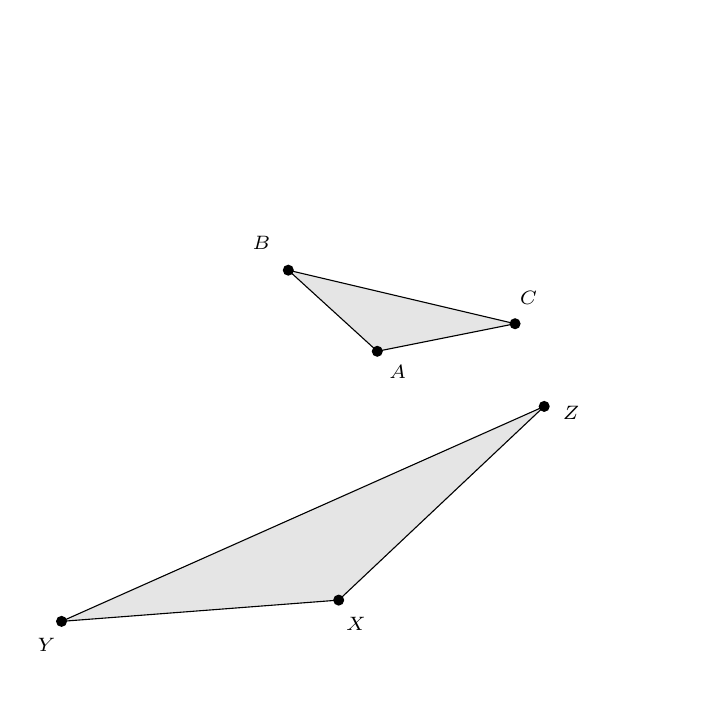
\begin{tikzpicture}[scale = 1]
    \clip(-6.42,-1.07) rectangle (2.01,7.25);
    \fill[fill=black,fill opacity=0.1] (-3.11,4.17) -- (-1.98,3.14) -- (-0.23,3.49) -- cycle;
    \fill[fill=black,fill opacity=0.1] (-5.99,-0.29) -- (-2.47,-0.02) -- (0.14,2.44) -- cycle;
    \draw (-3.11,4.17)-- (-1.98,3.14);
    \draw (-1.98,3.14)-- (-0.23,3.49);
    \draw (-0.23,3.49)-- (-3.11,4.17);
    \draw (-5.99,-0.29)-- (-2.47,-0.02);
    \draw (-2.47,-0.02)-- (0.14,2.44);
    \draw (0.14,2.44)-- (-5.99,-0.29);
    \begin{scriptsize}
        \fill [color=black] (-1.98,3.14) circle (2.0pt);
        \draw[color=black] (-1.72,2.88) node {$A$};
        \fill [color=black] (-3.11,4.17) circle (2.0pt);
        \draw[color=black] (-3.45,4.52) node {$B$};
        \fill [color=black] (-0.23,3.49) circle (2.0pt);
        \draw[color=black] (-0.06,3.82) node {$C$};
        \fill [color=black] (-2.47,-0.02) circle (2.0pt);
        \draw[color=black] (-2.25,-0.32) node {$X$};
        \fill [color=black] (-5.99,-0.29) circle (2.0pt);
        \draw[color=black] (-6.18,-0.59) node {$Y$};
        \fill [color=black] (0.14,2.44) circle (2.0pt);
        \draw[color=black] (0.48,2.36) node {$Z$};
    \end{scriptsize}
\end{tikzpicture}